\section{Introducci�n}
\label{s1:sec:Introduccion}

\subsection{El juego}
\label{s1:subsec:elJuego}
El videojuego \pong es uno de los videojuegos m�s conocidos por todos,
publicado por Atari en 1972. \pong consiste en un juego para dos personas,
en el que el objetivo es hacer rebotar a una pelota para que el oponente no
pueda golpearla y pierda.
\begin{figure}[h]
  \centering
  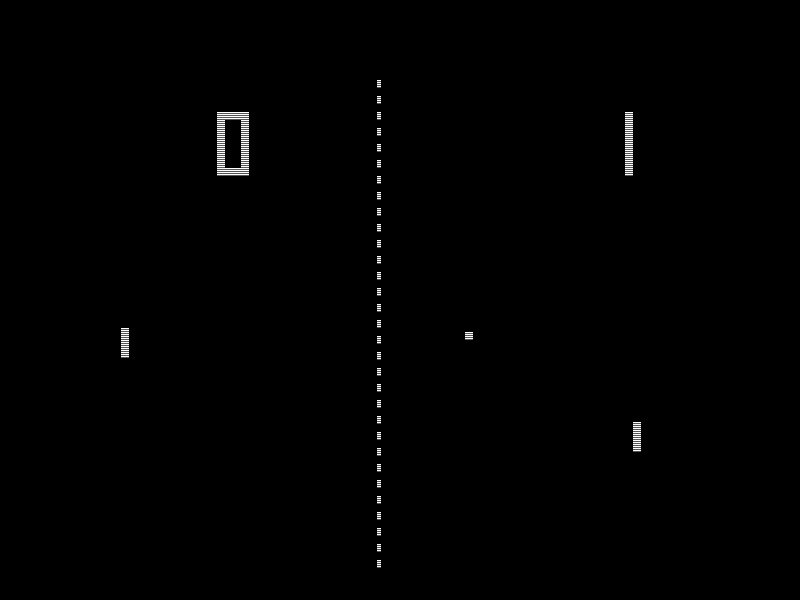
\includegraphics[width=0.4\textwidth]{images/pong.png}
  \caption{Imagen del juego original.}
  \label{s1:fig:pong}
\end{figure}

Para controlar la pelota, cada jugador dispone de una raqueta situada en
uno de los extremos de la pantalla. la cual �nicamente pude desplazarse en
vertical. Cuando la pelota golpea una de estas raquetas, esta cambia el
sentido horizontal de movimiento, dirigi�ndose al otro jugador. Seg�n en
que parte de la raqueta golpee la bola, esta tambi�n modifica su componente
de movimiento vertical. De igual manera, cuando la pelota golpea el borde
superior o inferior del juego, tambi�n ve modificado su movimiento.  Se
considera que un jugador pierde cuando no es capaz de golpear la pelota y
esta sale del juego por su lado de la pantalla.


\subsection{Descripci�n del proyecto}
\label{s1:subsec:objetivos}
El trabajo realizado consiste en el dise�o e implementaci�n del juego \pong
sobre una arquitectura distribuida formada por una FPGA Spartan~3~\cite{Spartan3}, y
dos maletines ARM S3C44B0X~\cite{maletinARM}, comunicados entre ellos
mediante UARTs.

La FPGA es el componente encargado de la l�gica del juego. En �l se
realizan todos los c�lculos de posiciones y choques de la pelota. Tambi�n
se lleva control de las puntuaciones. Adem�s, sobre la FPGA se han
implementado dos m�dulos adicionales, uno encargado de la comunicaci�n con
los maletines mediante UARTs, y otro para mostrar el juego en un monitor
VGA.\\
Los maletines ARM son utilizados para leer los movimientos de los jugadores
(mediante \rev{pulsadores y teclado matricial}) y comunic�rselo a la FPGA
mediante una UART. Adem�s, por motivos de dise�o de la FPGA (s�lo posee un
puerto UART), los maletines est�n dise�ados para ser conectados en serie y
retransmitir los mensajes de un malet�n al siguiente, hasta llegar a la
FPGA. \rev{La puntuaci�n del juego tambi�n es mostrada por los \textit{display}
8-segmentos de la placa.}

En la figura figura~\ref{s1:fig:vista_general_sistema} se puede ver una
descripci�n general del sistema.\\

\begin{figure}[h]
  \centering
  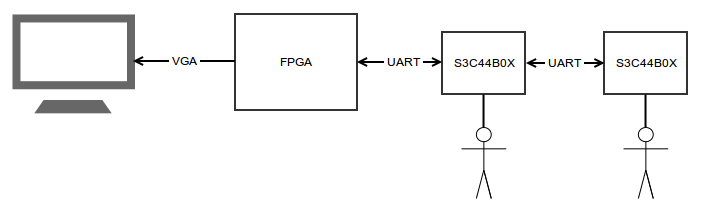
\includegraphics[width=0.8\textwidth]{images/descripcion_general.png}
  \caption{Descripci�n general del sistema.}
  \label{s1:fig:vista_general_sistema}
\end{figure}


\todo{REVISAR ESTO AL CABAR}\\
La memoria est� organizada de la siguiente forma:
la secci�n~\ref{21:sec:Disenyo} se muestra el modelado realizado por el
sistema, y diversos diagramas que describen el comportamiento del mismo. La
secci�n~\ref{s3:sec:Implementacion} muestra los aspectos m�s relevantes en
la implementaci�n. Y para finalizar, la secci�n~\ref{s4:sec:Conclusiones}
muestra unas conclusiones y trabajo futuro a realizar si se desea seguir
con el proyecto.








%
%
%%%
%%% Local Variables:
%%% mode: latex
%%% TeX-master: "../main.tex"
%%% End:


